\chapter{Introduction}
\label{chapter:Introduction}
In the field of computer vison and pattern recognition, determining a
model from a finite set of samples or a complex image without prior
knowledge is an ill-posed problem. Due to the the ill-posedness, in
the sense that a unique model may not exist, models specifying a priori
knowledge play an very important role in solving many important
computer vision problems, such as object tracking, shape recognition,
pose estimation segmentation, edge detection, stereo matching and 3-D
reconstruction.

Some parametric curve models, also known as deformable models,
deformable templates, snakes, or active contours, have been delevoped
to guides the image interpretation process towards particularly
likely interpretations(CCD). These parametric curve models, namely
prior knowledge have two main outstanding influences in the
development of related algorithms. First is the snakes which
represented a fundamentally new framework for delineating an object
outline in an image. This framework attempts to minimize an energy
associated to the current contour as a sum of an internal and external
energy(wikipedia). The goal of snakes is to balance the prior
knowledge with evidence from an image. The second outstanding
influence is in the field of pattern recognition and machine learning
where statistical distributions play key roles.  There treatment
of prior knowledge about shape is put into a probabilistic
context. Any shape is regarded as the result of applying some
distortion to an ideal prototype shape, and an appropriate
distribution governs the nature and extent of the distortion.
For both kinds of method, the common aim is to strengthen the visual
interpretation of shape via the stabilising influence of prior
expectations of the shapes that are likely to be seen.(AC 53) This
paper concerns the Contracting Curve Density (CCD) algorithm whose
basic step is solving a curve fitting problem in a probabilistic
context.


\section{The CCD algorithm and curve fitting problem}
\label{sec:ccdcfp}
Curve fitting is such a process that makes
a practical deformable templates (model) attach to the feature in a
image. It in essence involves using algorithms to find the parameter
values for a given parametric curve model. A lot of important and
challenging computer vision tasks can be formulated as variants of the
curve-ftting problem. The nature of curve fitting problem is taken into account from the
outset, usually it is quite unnecessary to examine an entire
image. Hence, there is no need to organise or group features in the
image, and the analysis can be restricted to a relatively narrow
ROI (region of interest), so it is usually expected to be computationally
cheaper.

The CCD algorithm can be described as follows. Given one or multiple images as input
data and a parametric curve model with a prior distribution of the model
parameters, through curving fitting process we estimate the model
parameters which determine the approximation of the posterior
distribution in order to make the curve model best match the image data.
Figure 1 depicts a curve-fitting problem and the corresponding solution obtained by the
CCD algorithm. 
\begin{figure}[htb]
  \centering
  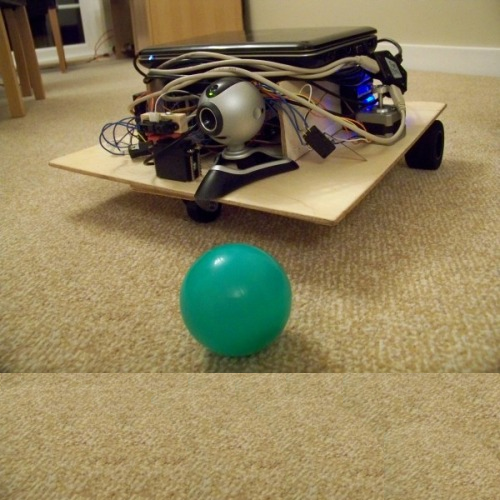
\includegraphics[width=10cm]{images/ball.png}
  \caption{\label{fig:1}}
\end{figure}



\section{Motivation of the CCD Approach}
\label{sec:mccd}
Curve fitting problem and its variant have a wide range of
applications in the field of robotics, medical processing, user
interface, surveillance and biometrics (hanek's paper). In order to be
widely applicable to practical computer vision problems, following
requirements, such as Robustness,
accuracy, efficiency, any-time property and versatility, should be
considered when a novel approach is designed and implemented.
However, in the computer vision community, solving object segmentation and the
related object contour tracking problem are always challenging, especially in natural and unconstrained scenes. Due to clutter,
shading, texture, and highlights it is very difficulty to segment
an object from an inhomogeneous background. Furthermore, some physical
conditions, such as the illumination or surface properties, will
influence the efficiency and stability of related approaches. It is
necessary and important to develop a method to determine adequate segmentation
criteria in advance or even and a single criteria that is applicable
for all parts of an object boundary.

Among the currently available methodologies, the CCD algorithm is an
interest one. It is developed and presented in as a state-of-the-art
improvement over other advanced techniques such as the condensation
algorithm (panin 2006). In the CCD approach, curve fitting problem is
put in the context of probabilistic framework and converted to a
regression one in the field of pattern recognition. It is especially
helpful to touch the nature of curving fitting problem. By introducing
local image statistics, the algorithm can cope with highly
inhomogeneous image regions and provide therefore locally adapted
criteria for separating the adjacent image regions. The use of blurred
curve models as efficient means for iteratively optimizing the
posterior density over possible model parameters. These blurred curve
models enable the algorithm to trade-off two conflicting objectives,
namely heaving a large area of convergence and achieving high
accuracy. The CCD algorithm achieves a high level of robustness and subpixel
accuracy even in the presence of severe texture, shading, clutter,
partial occlusion, and strong changes of illumination.(modify)



\section{The Contracting Curve Density (CCD) Approach}
\label{sec:sketch}

\subsection{Math description}
\label{sec:md}

In the field of pattern recognition, the key concept is that of
uncertainty. In a image, the uncertainty arises both
through noise on measurements, as well as through the nature of
objects. Probability theory provides a consistent framework for the
quantification and manipulation of uncertainty.  In this section, we
view curving fitting problem from a probabilistic perspective and talk
us towards to Bayesian treatment.

We assume a parametric curve model is governed by a prior distribution
over the model parameters $\Phi$ (usually a $D$-dimensional
vector). There exists a range of probability distributions which can
be used to model the distribution of shapes. In this thesis, for
simplicity, let us consider a Gaussian distribution, which is commonly
used in computer vison because of its several outstanding features.

% \begin{equation}
%   \label{eq:1.1}
%   p(\mathbf{\Phi} | \mathbf{m}_{\mathbf{\Phi}}, \mathbf{\mathbf{\Sigma}}_{\mathbf{\Phi}}) = \mathcal{N}(\mathbf{\Phi} |
%   \mathbf{m}_{\mathbf{\Phi}},\mathbf{\Sigma}_{\mathbf{\Phi}}) =
%   \frac{1}{(2\pi )^{D/2}} \frac{1}{|\mathbf{\Sigma}_{\mathbf{\Phi}}|^{1/2}}
% \mathrm{exp} \left\{ -\frac{1}{2} (\mathbf{\Phi} -
%   \mathbf{\Sigma}_{\mathbf{\Phi}})^T \mathbf{\Sigma}_{\mathbf{\Phi}}^{-1} (\mathbf{\Phi} -
%   \mathbf{\Sigma}_{\mathbf{\Phi}}) \right\}
% \end{equation}
% where the $D$-dimensional vector $\mathbf{m}_{\mathbf{\Phi}}$ is
% called the mean, the $D \times D$ matrix
% $ \mathbf{\Sigma}_{\mathbf{\Phi}} $ is called
% the covariance, and $|\mathbf{\Sigma}_{\mathbf{\Phi}}|$ denotes the
% determinant of $\mathbf{\Sigma}_{\mathbf{\Phi}}$

Defining the prior distribution is only the part of the problem. Prior knowledge
defines the possibility of shape in an image, if we want to know what
shape is presented in a given image, we must find the posterior
distribution. According the Bayesian theorem, posterior distribution
is proportional to the product of prior distribution and likelihood
function. Hence, the next step is define the likelihood function.

In the implementation of the CCD algorithm, it is suggested to use local image pixels $\mathcal{L}$ as the training data to
determine the likelihood function. If the data are assumed to be drawn
 independently from the distribution, then the likelihood function is
given by the accumulation of all components.
In this paper, by pixel value we denote the vector containing the local single-or multichannel
image data associated to a pixel. In our experiments, we directly use the sensed RGB
values as pixel values. However, other types of local features computed in a pre-processing
step may also be used, e.g. texture descriptors or color values in
other color spaces.

With the prior distribution and posterior distribution, now we can
apply the Bayesian treatment to the curve fitting problem.
We determine $\hat{\mathbf{\Phi}}$ by finding the most probable
value of $\mathbf{\Phi}$ given the data, in other words by maximizing
the posterior distribution. This technique is called maximum
posterior, or simply MAP.

There are several methods to estimate the MAP.
\begin{itemize}
\item in some special case, posterior distribution can be given in
  closed form analytically. This requires conjugate priors.
\item numerical optimization such as the conjugate gradient method or
  Newton's method.
\item modification of an expectation-maximization (EM) algorithm,
  which does not require to derive the posterior density.
\item Monte Carlo method using simulated annealing
\end{itemize}

In this thesis, we adopt the second method to obtain the MAP estimate.
Usually, the result is some parameters (e.g. mean and covariance) to
govern the posterior distribution. With the resulting parameters we
can predict what shape is actually likely to be present in a particular image.


\subsection{Possible problems}
\label{sec:prob}
In order to implement the MAP estimation above, we have to address
four three questions.

\begin{itemize}
\item How to create a parametric curve model as prior knowledge , and
  at same time determine the distribution? There are a variety of
  forms active shape models available, such as principally snakes,
  deformable templates and dynamic contours. For curve fitting
  problem, deformable template is a good choice to match the image
  data. Then we have to choose suitable number of parameters to control
  the strength of prior assumptions. If there are too many parameters
  in the model, it is easy to control the contour accurately at the
  expense of complexity and computational cost. Balance among these
  aspects are non-trivial.

\item How can the local statistics in the image evaluated? First, it
  is necessary to establish the relation between model parameters
  $\mathbf{\Phi}$ and the image data $\mathcal{L}$. This is a especially
challenging in the presence of clutter and strong texture if we
consider the factors, such as  illumination, surface properties ,
characteristics of the camera and shadow. 

\item How can the fit be optimized efficiently? Generally MAP and some
  other nonlinear optimization algorithms may find multiple local maxima and are not guaranteed to find the
  largest of these maxima.
\end{itemize}


For the first question, we will use parametric B-Spline curve as
our prior knowledge. It is proved that this kind of curve model is
flexible enough and can well represent the contour of object. The
parametric B-Spline curve will be described in the chapter 3.
The second question is especially challenging. In order to simplify
the problem, it is necessary to make some assumptions about the image
data. we will describe such assumptions in more detail. For the last
question, different optimization methods used for curve-fitting will
be discussed in this thesis.

\subsection{Sketch of the CCD algorithm}
\label{sec:sccd}

In this section, the basic steps of the CCD algorithm will be sketched.

Given an input image as training data, we first choose an initial
contour for an object or feature which will be fitted or tracked, and
some initial values for the means, covariances. Then we alternatively
between the following two updates that we shall call the learning
local statistics step and the refining parameters step, for reasons
that will become apparent shortly.
In the step of learning local statistics, for each pixel $\nu$ in the
vicinity of the expected curve, two sets of local statistics
are computed, one set for each side of the curve. The local statistics are obtained from
pixels that are close to pixel $nu$ and most likely lie on the corresponding side of the curve,
according to the current estimate of the model parameters. The resulting local statistics
represent an expectation of "what the two sides of the curve look
like".(Hanek's paper)

The CCD algorithm has some interesting similarities to the Expectation-Maximization
(EM) algorithm (Dempster et al., 1977), which is often used for clustering-based image
segmentation, a subset of region-based image segmentation (Hermes et al., 2002; Belongie
et al., 1998). The first step computes local statistics defining an expectation of the pixel
values (E-step). The second step maximizes this expectation
(M-step). The CCD algorithm differs mainly by: 1.) using local
statistics, 2.) exploiting a curve model and optimizing model
parameters rather than pixel classifications.


\section{Overview of the Thesis}
\label{sec:overview}
The remainder of this paper is organized as follows. In Chapter 2,
related work on PR2, Robot Operation System (ROS), active contour,
some curve-fitting ,image segmentation and tracking algorithms will be
introduced. Details on shape-space models and parametric
B-Spline curves are discussed in chapter 3. In chapter 4 , we give a brief introduction of software
and hardware infrastructure used in the implementation of the CCD
approach. We will concern the OpenCV library, ROS and PR2, and chapter
5 explain the CCD approach in detail. This will be followed by a
description of the application of the CCD approach in
robotics. In chapter 7, experiments and results are given. In
addition, we evaluate the performance of the CCD algorithm and the CCD
tracker in terms of robustness, accuracy, and runtime. In chapter 8,
the work of this thesis is concluded with the future work for improvement.


